% Use the Research-project-manuscript-template class directly.
\documentclass[onecolumn]{../../../../../template/Research-project-manuscript-template/main}

% Local Springer-like extension: use the template's centered journal title
% block without the decorative card used by the fancy style.
\makeatletter
\newcommand{\sa@maketitle@springer}{%
  \begingroup
    \sa@simple@titleblock@typography
    \begin{center}
      {\huge\sffamily\bfseries\color{titlefg}\nohyphens\sa@title\par}
      \vskip 0.35cm
      {\setstretch{1.0}\normalsize\sa@authorlist\par}
      \ifdefempty{\sa@affiliationlist}{}{\vskip 0.16cm{\sa@affiliationlist\par}}%
      \ifdefempty{\sa@contributionlist}{}{\vskip 0.12cm{\sa@contributionlist\par}}%
    \end{center}
    \ifdefempty{\sa@abstract}{}{%
      \vskip 0.20cm
      {\color{rulecolor!65}\rule{\linewidth}{0.45pt}}\par\vskip 0.18cm
      \sa@printabstract
    }%
    \ifdefempty{\sa@keywords}{}{%
      \vskip 0.12cm
      {\setstretch{1.08}\small\rmfamily\color{inkfg}\bfseries Keywords:\mdseries\enspace\sa@keywords\par}%
    }%
    \ifdefempty{\sa@metadatalist}{}{%
      \vskip 0.18cm
      {\centering\setstretch{1.0}\small\sa@metadatalist\par}%
    }%
  \endgroup
  \FloatBarrier
}
% In the template's simple style, make the complete keyword line match the
% abstract typography (small roman type and the same line spacing).
\patchcmd{\sa@maketitle@simple}
  {{\normalsize\sffamily\textbf{\color{titlefg}Keywords:}\enspace\color{titlefg}\sa@keywords\par}}
  {{\setstretch{1.08}\small\rmfamily\color{inkfg}\bfseries Keywords:\mdseries\enspace\sa@keywords\par}}
  {}{\PackageWarning{main}{Could not patch simple-style keyword typography}}
\makeatother
\paperstyle{simple}
\papercolor{black}
\paperfont{times}
\papermanuscript{compact}
\papermode{final}
\paperanonymous{false}
\paperlinenumbers{false}
\paperbibliography{apa}

\title{Controlling LLM Agent Personality and Preferences through Representation Engineering}
\author[1]{Zeyu Lyu}
\author[1]{Zhichao Wang}
\affiliation[1]{Graduate School of Arts and Letters, Tohoku University}

\abstract{Large language model (LLM) agents offer a flexible approach to constructing ``silicon samples,'' with considerable potential for social science research. However, their behavior is often sensitive to prompt wording, difficult to interpret, and biased toward model-default preferences. We investigate activation steering as a means of controlling agent personalities and preferences by intervening in the model’s internal representations. Using Llama-3.1-8B-Instruct, we construct steering vectors and apply them during inference at varying scalar coefficients. We illustrate this approach through two proof-of-concept studies. First, we manipulate a latent personality trait and show that steering can systematically shift agents’ behavior across multiple behavioral games. Second, we manipulate a model-default preference and show that steering can alter both individual choices and collective norm trajectories. Our findings highlight the potential of representation engineering to enhance the interpretability and reproducibility of LLM-based social science research.}

\keywords{large language models; social simulation; activation steering; representation engineering; social norms}

\begin{document}
\maketitle

\section{Introduction}
LLM agents can generate context-dependent responses, assume heterogeneous profiles, and interact through natural language, making them promising ``silicon samples'' for surveys, experiments, and social simulations \citep{argyle2023,park2023,anthis2025}. However, prompt-based agents pose several methodological problems. First, small changes in instructions can alter agents' decisions, undermining the reproducibility of simulation results \citep{loya2023}. Second, pretrained and instruction-tuned models may converge on an ``average'' persona and therefore fail to represent meaningful heterogeneity across individuals \citep{argyle2023,bisbee2024,wang2025}. Third, model-default preferences may be mistaken for attitudes or norms that emerge through interaction, obscuring the distinction between pretrained tendencies and simulated social processes \citep{bail2024}. These problems of reproducibility and interpretability are especially salient in social science applications, where the goal is to understand the mechanisms underlying social phenomena and human behavior.

Representation engineering provides a promising approach to these challenges. The basic idea is that concepts and behavioral tendencies can be encoded as directions in a model's activation space and that modifying activations along these directions can systematically change generated behavior \citep{turner2023,konen2024}. Rather than specifying an agent solely through a persona prompt, activation steering manipulates a targeted internal representation while holding the task prompt constant. Specifically, we examine whether this approach can control an agent's personality and preferences sufficiently to create varied conditions for social simulation.

\section{Method}
The experiments use \texttt{meta-llama/Llama-3.1-8B-Instruct}. For a target property, we construct $N$ contrastive text pairs that differ in the relevant behavior or preference while remaining otherwise comparable. At model layer $l$, the steering vector is the mean activation difference
\begin{equation}
 \bm{v}^{(l)}=\frac{1}{N}\sum_{i=1}^{N}\left[\bm{a}^{(l)}(x_i^+)-\bm{a}^{(l)}(x_i^-)\right].
\end{equation}
During inference, the vector is added to the residual-stream activation,
\begin{equation}
 \bm{a}^{(l)}_{\mathrm{steered}}=\bm{a}^{(l)}+\alpha\bm{v}^{(l)},
\end{equation}
where the sign and magnitude of $\alpha$ determine the direction and strength of steering. This design keeps the decision prompt fixed and turns the targeted agent property into an explicit experimental parameter.

To manipulate a personality-related characteristic, we identify an altruism-related steering vector and use it to control agents' degree of altruism. Specifically, agents participate in the dictator, trust, ultimatum, and public goods games and explain their decisions. GPT-4 serves as an external evaluator, assigning each response an altruism rating on a scale from 0 to 100. This procedure allows us to measure the effect of steering on a latent personality trait across multiple tasks.

To manipulate a preference-related characteristic, we consider a simple social-norm scenario in which agents must choose between two payment schemes: sharing each payment equally or taking turns paying. The model exhibits a default preference for shared payment, which could constrain the range of outcomes in a social simulation. We therefore construct a rotating-payment steering vector to counteract this bias and examine how it affects individual choices and collective norm trajectories.

\begin{figure}[t]
  \centering
  \captionsetup[subfigure]{justification=centering,singlelinecheck=false}
  \begin{subfigure}[b]{0.375\textwidth}
    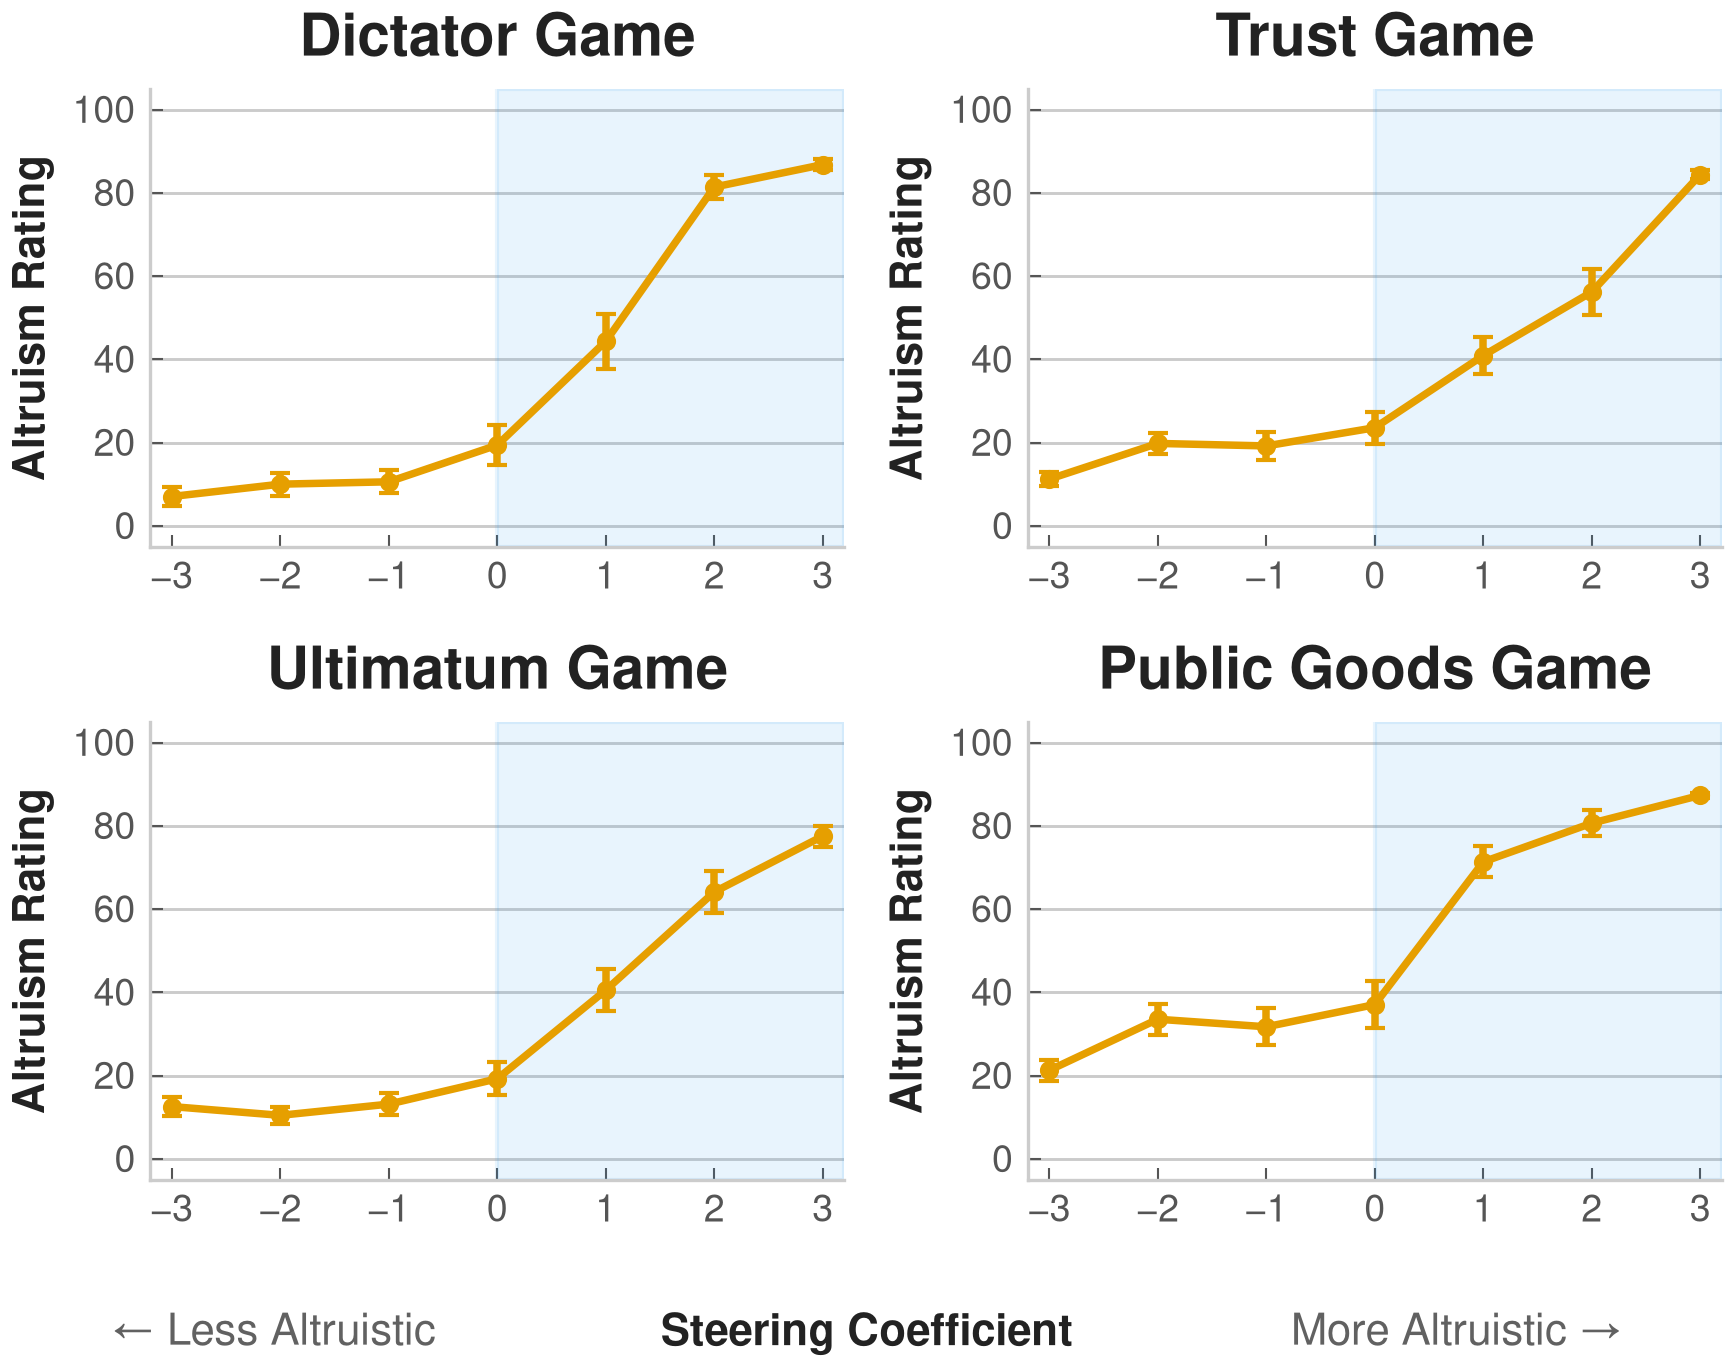
\includegraphics[width=\linewidth]{../image/figure3a_altruism_ratings_by_game-3.png}
    \caption{Effect of altruism steering on agents' altruistic behavior across behavioral games.}
  \end{subfigure}\hfill
  \begin{subfigure}[b]{0.615\textwidth}
    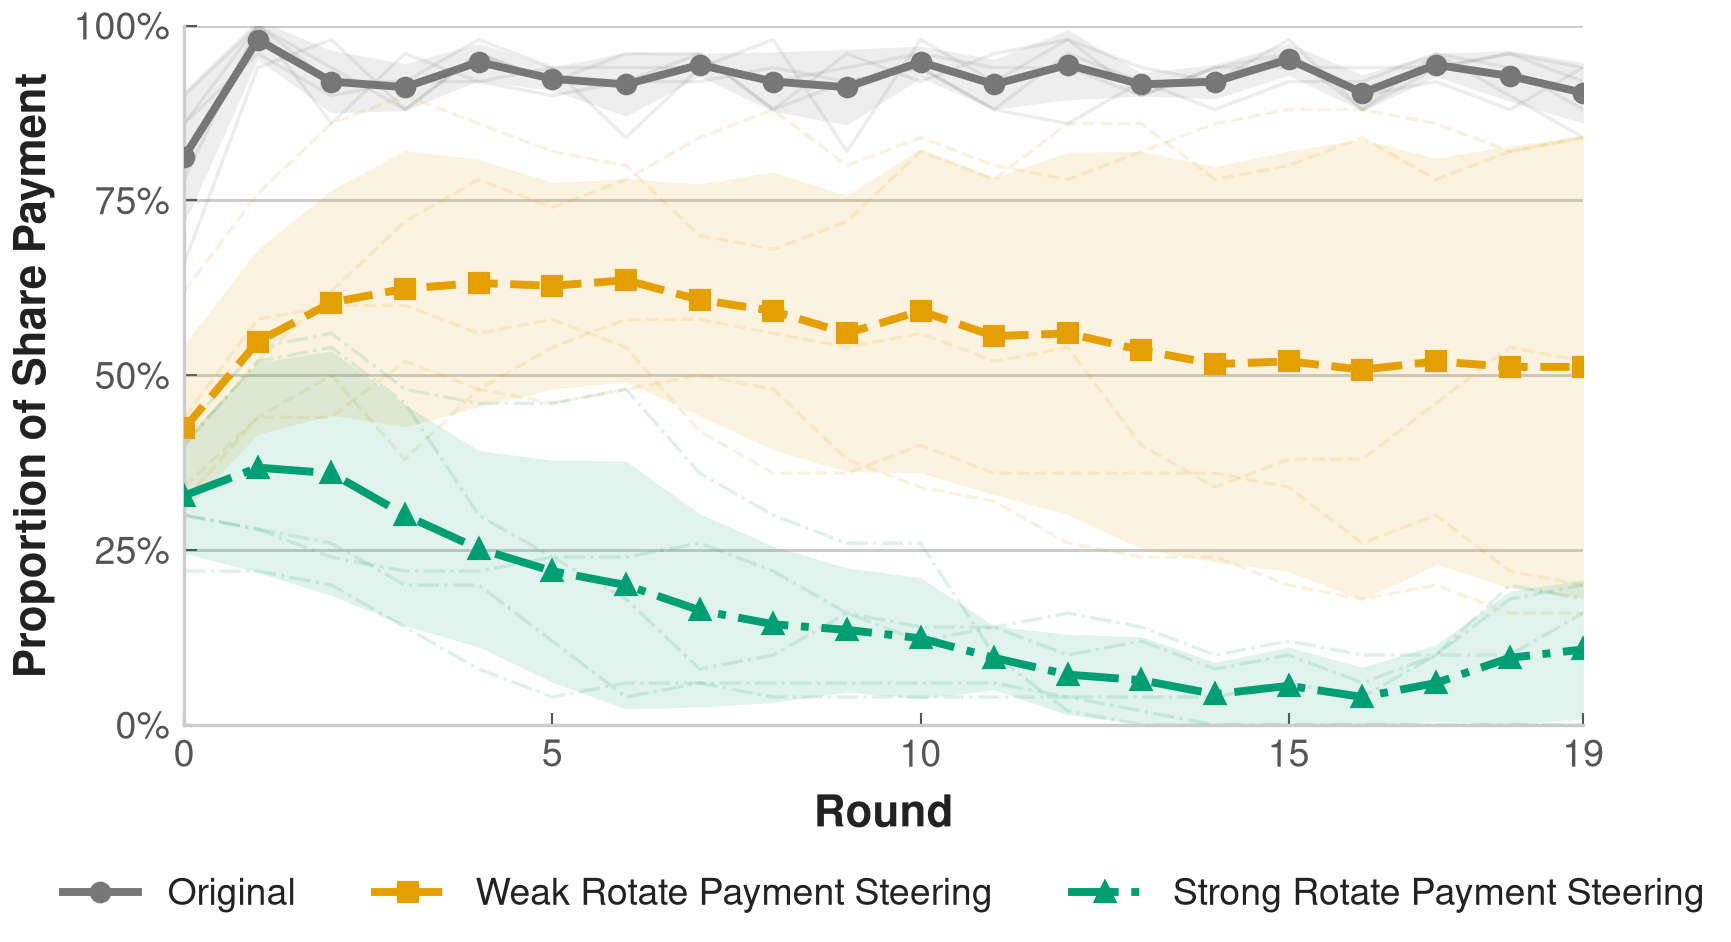
\includegraphics[width=\linewidth]{../image/m0_control_trajectories-3.png}
    \caption{Collective norm trajectories under different rotating-payment steering conditions.}
  \end{subfigure}
  \caption{Effects of activation steering on personality and preferences.}
  \label{fig:results}
\end{figure}

\section{Results}
\textbf{Altruism.} Figure~\ref{fig:results}a shows a clear dose--response relationship across the behavioral experiments. Negative coefficients, which steer agents toward less altruistic behavior, yield lower altruism ratings, whereas positive coefficients, which steer agents toward more altruistic behavior, yield higher ratings. This result demonstrates that activation steering can manipulate a latent personality trait across multiple tasks, providing a means of generating heterogeneous agent profiles in social simulations.

\textbf{Payment preferences and norm trajectories.} Agents are connected in a small-world network and, in each round, observe their neighbors' choices and update their own decisions based on prior commitment and social influence; the resulting simulation trajectories are therefore sensitive to agents' initial preferences, which can be controlled using the steering vector.

The unsteered model displays a pronounced default preference for shared payment, as evidenced by the high proportion of shared-payment choices across rounds. Applying rotating-payment steering counteracts this bias and alters both individual choices and collective norm trajectories. Manipulating the strength of agents' prior commitment further reveals how this factor interacts with steering: the steering vector shifts agents' payment preferences, producing different norm trajectories under otherwise comparable simulation rules.

\section{Discussion and Conclusion}
These results demonstrate two uses of representation engineering in social simulation. Activation steering can manipulate latent personality traits and model-default preferences in LLM agents, providing a tool for generating heterogeneous agent profiles and controlling simulation conditions. Compared with prompt-based methods, this approach may improve interpretability and reproducibility by allowing researchers to manipulate internal representations explicitly while holding the task prompt constant.

These findings should nevertheless be interpreted as a proof of concept rather than as evidence that activation steering generalizes automatically. Our experiments use one model and two target properties, and the intervention depends on the contrastive examples used to estimate the direction, the layer at which it is applied, and the coefficient controlling its strength. More broadly, systematic evaluations have found substantial variation in steering effectiveness across model families, with some interventions producing no improvement or even degrading performance \citep{dasilva2025}. Future work should therefore test whether steering vectors transfer across models, prompts, and simulation tasks; evaluate unintended changes in non-target behaviors; and develop more robust procedures for selecting contrastive data, layers, and coefficients.

\bibliographystyle{\paperbibstyle}
\bibliography{references}
\end{document}
